\section{Introduction} \label{section: intro and motiv}

\begin{wrapfigure}{r}{0.45\textwidth}
\vspace{-1.5cm}
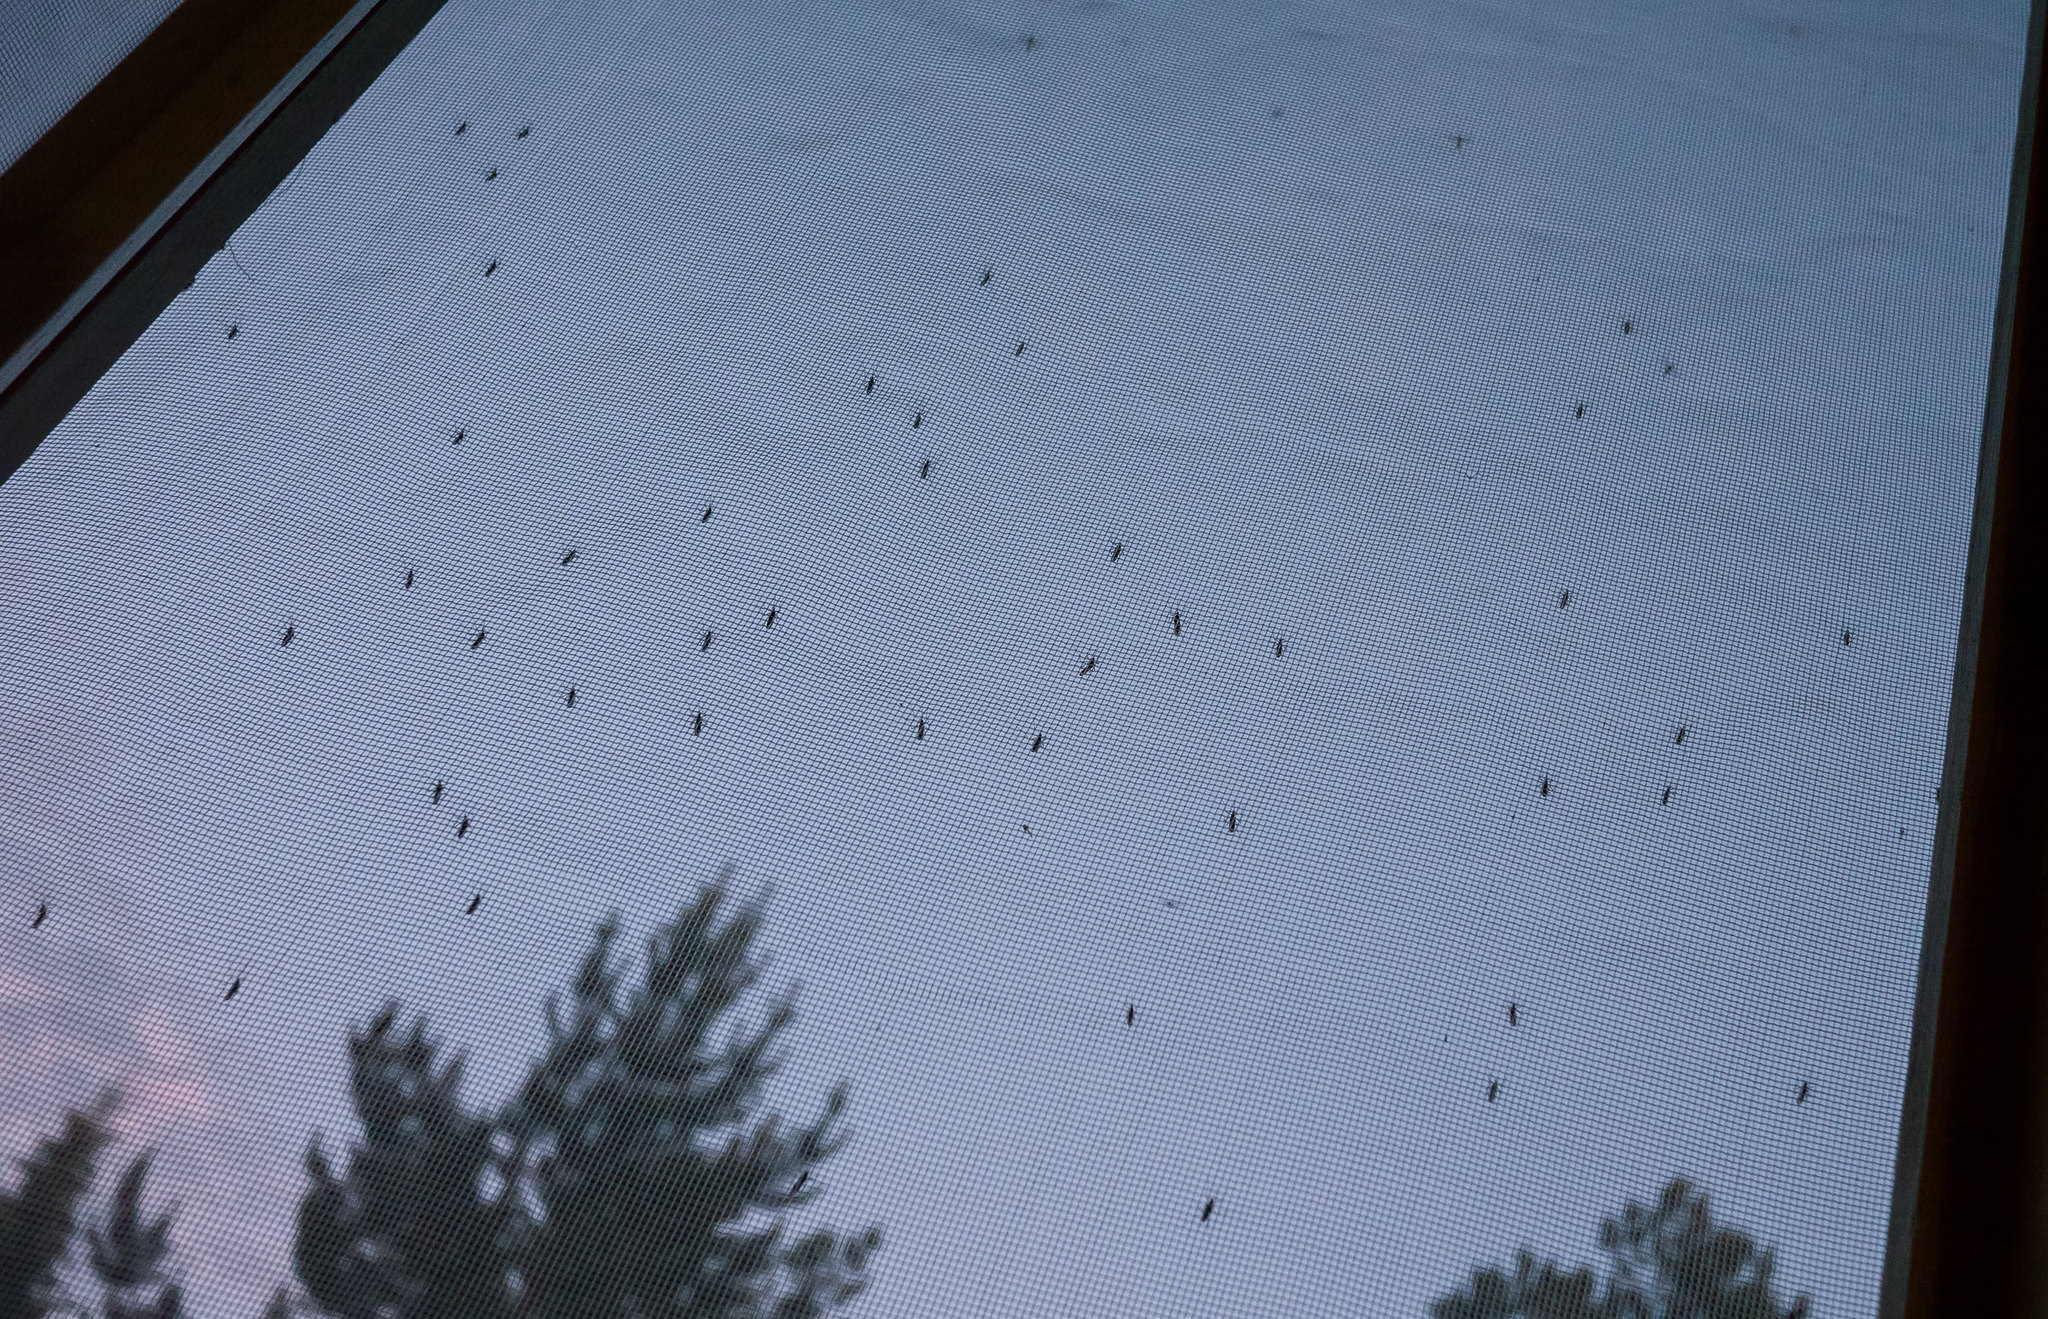
\includegraphics[width=0.9\linewidth]{figures/mosquitogrid.jpg}
\caption{Anti-bug grid (\href{https://www.flickr.com/photos/neekohfi/7817306994/}{Flickr.com})}\
\end{wrapfigure}

Bug grids can be placed over open windows to allow air to flow through without letting bugs into someone's house. Presumably, when people open their windows, they want air to flow through their house. However, our hypothesis is that a bug grid will decrease the flux and that different grids will affect the flux differently. Using a fluid flow simulation, we want to study how the grid's thickness and hole density affect the flux. Finding optimal thickness and hole density can help design anti-bug grids.

\subsection{Research question}
\textbf{Main:}
\begin{itemize}
    \item How much does the air flux through a window with a bug grid change with the grid's thickness and density?
\end{itemize}
\textbf{Subquestions:}
\begin{itemize}
    \item What are the optimal parameters of the grid that maximise airflow while keeping the bugs out?
    \item In which section of the window has the airflow decreased the most due to the presence of the bug grid?
\end{itemize}
